\chapter{Heian Vengeful Spirits: Onryō and Goryō}

\section{A capital full of spirits}

The Heian capital (Kyoto, founded 794) was laid out on a Chinese grid and protected by
careful geomancy, yet its aristocrats lived in constant fear of spirits. Illness, fires,
lightning, epidemics and the deaths of princes were routinely attributed to the anger of the
dead. The capital itself was moved from Nagaoka to Heian partly because of the angry ghost
of Prince Sawara (d.\ 785), who had died protesting his innocence.

\begin{definition}[Onryō and goryō]
An \emph{onryō} (\ja{怨霊}) is the spirit of a person who died with a grudge (\ja{怨み},
urami), especially through injustice, and who returns to harm the living. When such a
spirit is officially pacified and worshipped, it becomes a \emph{goryō} (\ja{御霊},
``honourable spirit''). The \emph{goryō-e} (\ja{御霊会}) were rituals held from 863 to
appease such spirits; the Gion festival in Kyoto began as one.
\end{definition}

\begin{center}
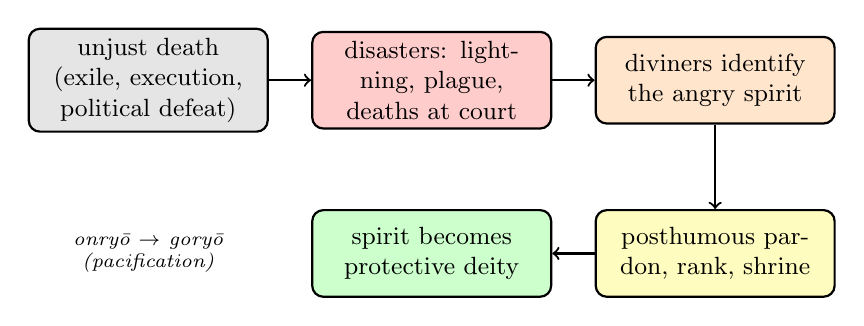
\begin{tikzpicture}[b/.style={draw, thick, rounded corners, align=center, font=\small, text width=2.8cm, minimum height=1.1cm}]
  \node[b, fill=gray!20] (a) at (0,0) {unjust death\\(exile, execution, political defeat)};
  \node[b, fill=red!20] (b) at (3.6,0) {disasters: lightning, plague, deaths at court};
  \node[b, fill=orange!20] (c) at (7.2,0) {diviners identify the angry spirit};
  \node[b, fill=yellow!25] (d) at (7.2,-2.2) {posthumous pardon, rank, shrine};
  \node[b, fill=green!20] (e) at (3.6,-2.2) {spirit becomes protective deity};
  \draw[->, thick] (a) -- (b); \draw[->, thick] (b) -- (c); \draw[->, thick] (c) -- (d);
  \draw[->, thick] (d) -- (e);
  \node[font=\scriptsize\itshape, align=center] at (0,-2.2) {onryō $\to$ goryō\\(pacification)};
\end{tikzpicture}
\end{center}

\section{Sugawara no Michizane (845--903)}

\subsection{Life}

Michizane was a brilliant scholar of Chinese learning and poet from a family of modest
rank. He rose under Emperor Uda to become Minister of the Right, an unusual position for a
non-Fujiwara. In 894 he recommended ending the embassies to Tang China. In 901 his Fujiwara
rival, Fujiwara no Tokihira, had him falsely accused of plotting and exiled to Dazaifu in
Kyushu, where he died in misery in 903.

\begin{aside}
Before leaving the capital he wrote a famous poem to the plum tree in his garden: ``When
the east wind blows, send me your fragrance, plum blossoms; though your master is gone, do
not forget the spring.'' Legend says the tree flew to Dazaifu to join him (the
``flying plum'', \ja{飛梅}, tobiume).
\end{aside}

\subsection{The haunting}

\begin{center}
\begin{tabular}{lp{10.5cm}}
\toprule
Year & Event attributed to Michizane's spirit \\
\midrule
908 & death of Fujiwara no Sugane, one of the accusers \\
909 & death of Tokihira at age 39 \\
913 & death of Minamoto no Hikaru, another conspirator (drowned while hunting) \\
923 & death of the crown prince (Tokihira's nephew); Michizane posthumously restored to office \\
925 & death of the next crown prince, aged five \\
930 & lightning strikes the Seiryōden palace hall, killing several courtiers; Emperor Daigo dies three months later \\
\bottomrule
\end{tabular}
\end{center}

\subsection{Becoming Tenjin}

Michizane was identified with the \textbf{thunder god}. In 947 the Kitano Tenmangū shrine
was founded in Kyoto, and in 993 he was granted the highest posthumous rank. He became
\textbf{Tenjin} (\ja{天神}, ``heavenly deity''), worshipped today as the god of
\emph{scholarship}. Every winter, students preparing for entrance exams visit Tenmangū
shrines and buy charms and wooden prayer plaques (\ja{絵馬}, ema).

\begin{important}[Exam point]
The arc of Michizane is the model case of onryō $\to$ goryō: a wronged man becomes a
terrifying spirit, is pacified through rank and worship, and ends as a benevolent deity
connected to his talent in life (scholarship). His fury is not denied but \emph{redirected}.
\end{important}

\section{Taira no Masakado (d.\ 940)}

Masakado was a warrior in the eastern Kantō who rebelled against the court, seized
several provinces and proclaimed himself the ``New Emperor'' (\ja{新皇}, shinnō) in 939. He
was killed in 940 by Fujiwara no Hidesato and Taira no Sadamori.

\begin{itemize}
  \item \textbf{The head}: his head was displayed in Kyoto, where (in legend) it stayed
        fresh for months, its eyes open, shouting for its body. One night it flew back east
        and fell to earth in what is now Ōtemachi, Tokyo.
  \item \textbf{Kubizuka} (\ja{首塚}, ``head mound''): a small monument to his head stands
        among the skyscrapers of Tokyo's financial district. Attempts to move or build over it
        are said to have caused deaths (the Ministry of Finance after the 1923 earthquake;
        an accident during the US occupation when bulldozers tried to clear it).
        Neighbouring office workers reportedly arrange desks so as not to turn their backs
        to it.
  \item \textbf{Kanda Myōjin}: Masakado is one of the deities of this major Tokyo shrine,
        a protector of Edo/Tokyo.
\end{itemize}

\begin{remark}
In Aramata Hiroshi's novel \emph{Teito Monogatari} (1985) and its film adaptation, the
villain Katō tries to awaken Masakado's spirit to destroy Tokyo. Masakado is the
``guardian/destroyer of Tokyo'' figure in modern fiction, comparable to Godzilla.
\end{remark}

\section{Possession in \emph{The Tale of Genji}}

In Heian literature the most famous spirit is not a dead man but a living woman. In
\emph{Genji}, Lady Rokujō, an older, proud lover whom Genji neglects, unknowingly sends out
her spirit as an \emph{ikiryō} (\ja{生霊}, ``living spirit'') that kills Genji's lover
Yūgao and later possesses and kills his wife Aoi.

\begin{example}[The carriage quarrel]
At the Kamo festival, servants of Genji's wife Aoi push Rokujō's carriage out of the way and
damage it. The public humiliation turns her jealousy into a spirit that attacks Aoi in
childbirth. Exorcists transfer the spirit into a medium (\ja{憑坐}, yorimashi) to
identify it. Later the Noh play \emph{Aoi no Ue} shows Rokujō with the mask of the
\emph{hannya} (\ja{般若}), a horned woman-demon of jealousy.
\end{example}

\begin{important}[Gender and the vengeful spirit]
Male onryō (Michizane, Masakado) are political: wronged ministers and rebels. Female
spirits tend to be driven by \emph{jealousy} and \emph{love}, and their violence is aimed at
rival women. This gendered pattern becomes the basis for Edo-period ghost stories (Oiwa,
Week 5) and J-horror (Sadako, Week 10).
\end{important}

\section{Abe no Seimei and onmyōdō}

The Bureau of Yin and Yang (\ja{陰陽寮}, Onmyōryō) employed court diviners who read the
calendar and the stars, identified spirit attacks and performed exorcisms. The most famous
was \textbf{Abe no Seimei} (921--1005).

\begin{itemize}
  \item Legends: his mother was a white fox (Kuzunoha), which explains his supernatural
        powers (see Week 6 on kitsune). He commanded twelve servant spirits
        (\ja{式神}, shikigami), which he hid under a bridge because his wife feared them.
  \item His rivalry with the evil diviner Ashiya Dōman is the subject of many tales.
  \item Popular revival: Yumemakura Baku's \emph{Onmyōji} novels (from 1986), a manga by
        Okano Reiko and the 2001 film starring Nomura Mansai made Seimei a 1990s--2000s pop
        hero. His symbol is the five-pointed star (\ja{晴明桔梗}).
\end{itemize}

\begin{center}
\begin{tikzpicture}[b/.style={draw, thick, rounded corners, align=center, font=\small, minimum width=2.6cm}]
  \node[b, fill=purple!15] (s) at (0,0) {\textbf{Onryō}\\\ja{怨霊}};
  \node[b, fill=blue!10] (m) at (-4.5,1.4) {Michizane\\political, male};
  \node[b, fill=blue!10] (t) at (-4.5,-1.4) {Masakado\\rebel, male};
  \node[b, fill=red!10] (r) at (4.5,1.4) {Rokujō (\emph{ikiryō})\\jealous, female};
  \node[b, fill=red!10] (o) at (4.5,-1.4) {Oiwa, Sadako\\(later periods)};
  \node[b, fill=yellow!20] (seimei) at (0,-2.4) {response: onmyōji, monks,\\shrines (pacification)};
  \draw[->, thick] (m) -- (s); \draw[->, thick] (t) -- (s);
  \draw[->, thick] (r) -- (s); \draw[->, thick, dashed] (o) -- (s);
  \draw[->, thick] (s) -- (seimei);
\end{tikzpicture}
\end{center}

\section*{Summary}
\begin{itemize}
  \item Heian aristocrats attributed disasters to onryō, spirits of the wrongfully dead.
  \item Pacification (goryō rites, rank, shrines) turns them into protective deities.
  \item Michizane $\to$ Tenjin (scholarship); Masakado $\to$ protector of Tokyo with his
        haunted head mound.
  \item Female spirits (Rokujō's ikiryō) are driven by jealousy: the template for later
        ghost women.
  \item Onmyōji like Abe no Seimei managed spirits and became modern pop heroes.
\end{itemize}
